\documentclass{article}
\usepackage[utf8]{inputenc}
\usepackage{listings}
\usepackage{float}
\usepackage{graphicx}
\usepackage{fullpage}
\usepackage{caption}
\usepackage{subcaption}

\renewcommand{\thesubsection}{\arabic{subsection}}

\title{Pattern Recognition practical 1}
\author{Maikel Withagen \and Steven Bosch}
\date{September 2015}
\lstset{frame=single}

\begin{document}

\maketitle

\section{Assignment 1}
\subsection{}
Consider it done
\subsection{}
To compute the pair-wise correlation coefficients we used the following command:
\begin{lstlisting}[title= Input]
load('lab1_1.mat')
corrcoef(lab1_1)
\end{lstlisting}
This yields us the following table of correlation coefficients:
%\begin{lstlisting}[title= Output]
%   1.0000   -0.0615    0.7156
%  -0.0615    1.0000    0.5142
%   0.7156    0.5142    1.0000
%\end{lstlisting}
\begin{table}[H]
\caption{\textit{Pair-wise correlation coefficients}}
\vspace{0.1cm}
\centering
\begin{tabular}{|c|c|c|c|}
\hline
 & Length & Age & Weight \\
\hline
Length & 1 & -0.0615 & 0.7156 \\
\hline
Age & -0.615 & 1 & 0.5142 \\
\hline
Weight & 0.7156 & 0.5142 & 1 \\ 
\hline
\end{tabular}
\label{tab1.2}
\end{table}

\subsection{}

\begin{figure}[H]
\centering

\begin{subfigure}[b]{.45\linewidth}
The two features for which the correlation is the largest are the first and third column, respectively the height and the weight.
\centering
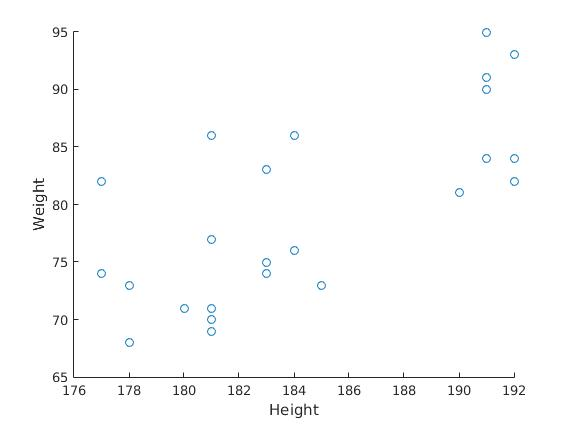
\includegraphics[width=\columnwidth]{plot_1_3_a.jpg}
\caption{Scatterplot of weight to length}
\label{fig1.3a}
\end{subfigure}%
\quad
\begin{subfigure}[b]{.45\linewidth}
The two features for which the correlation is the second largest are the second and third column, respectively the height and the weight.
\centering
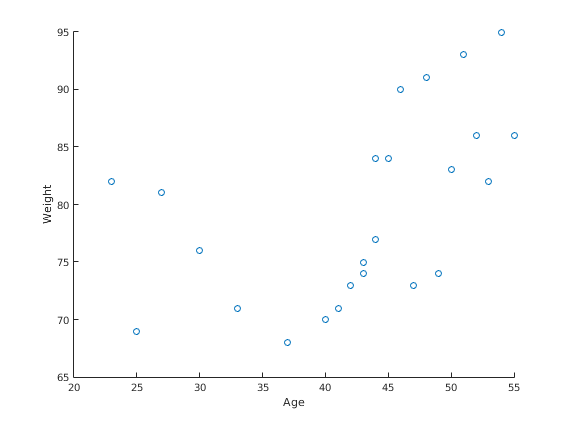
\includegraphics[width=\linewidth]{plot_1_3_b.png}
\caption{Scatterplot of weight to age}
\label{fig1.3b}
\end{subfigure}
\caption{}
\end{figure}


From a scatterplot alone it is hard to draw conclusions about any possible relationships between the different features. 
We do get indications though; figure \ref{fig1.3a} shows that there is likely to be a correlation between the weight and the height.
An increase in weight seems to correspond to a (somewhat linear) increase in height. 
A similar kind of relationship can be seen in figure \ref{fig1.3b}, between the factors weight and age.

\section{Assignment 2}
\subsection{}

\subsection{}
\subsection{}
\subsection{}
\begin{figure}[H]
\centering
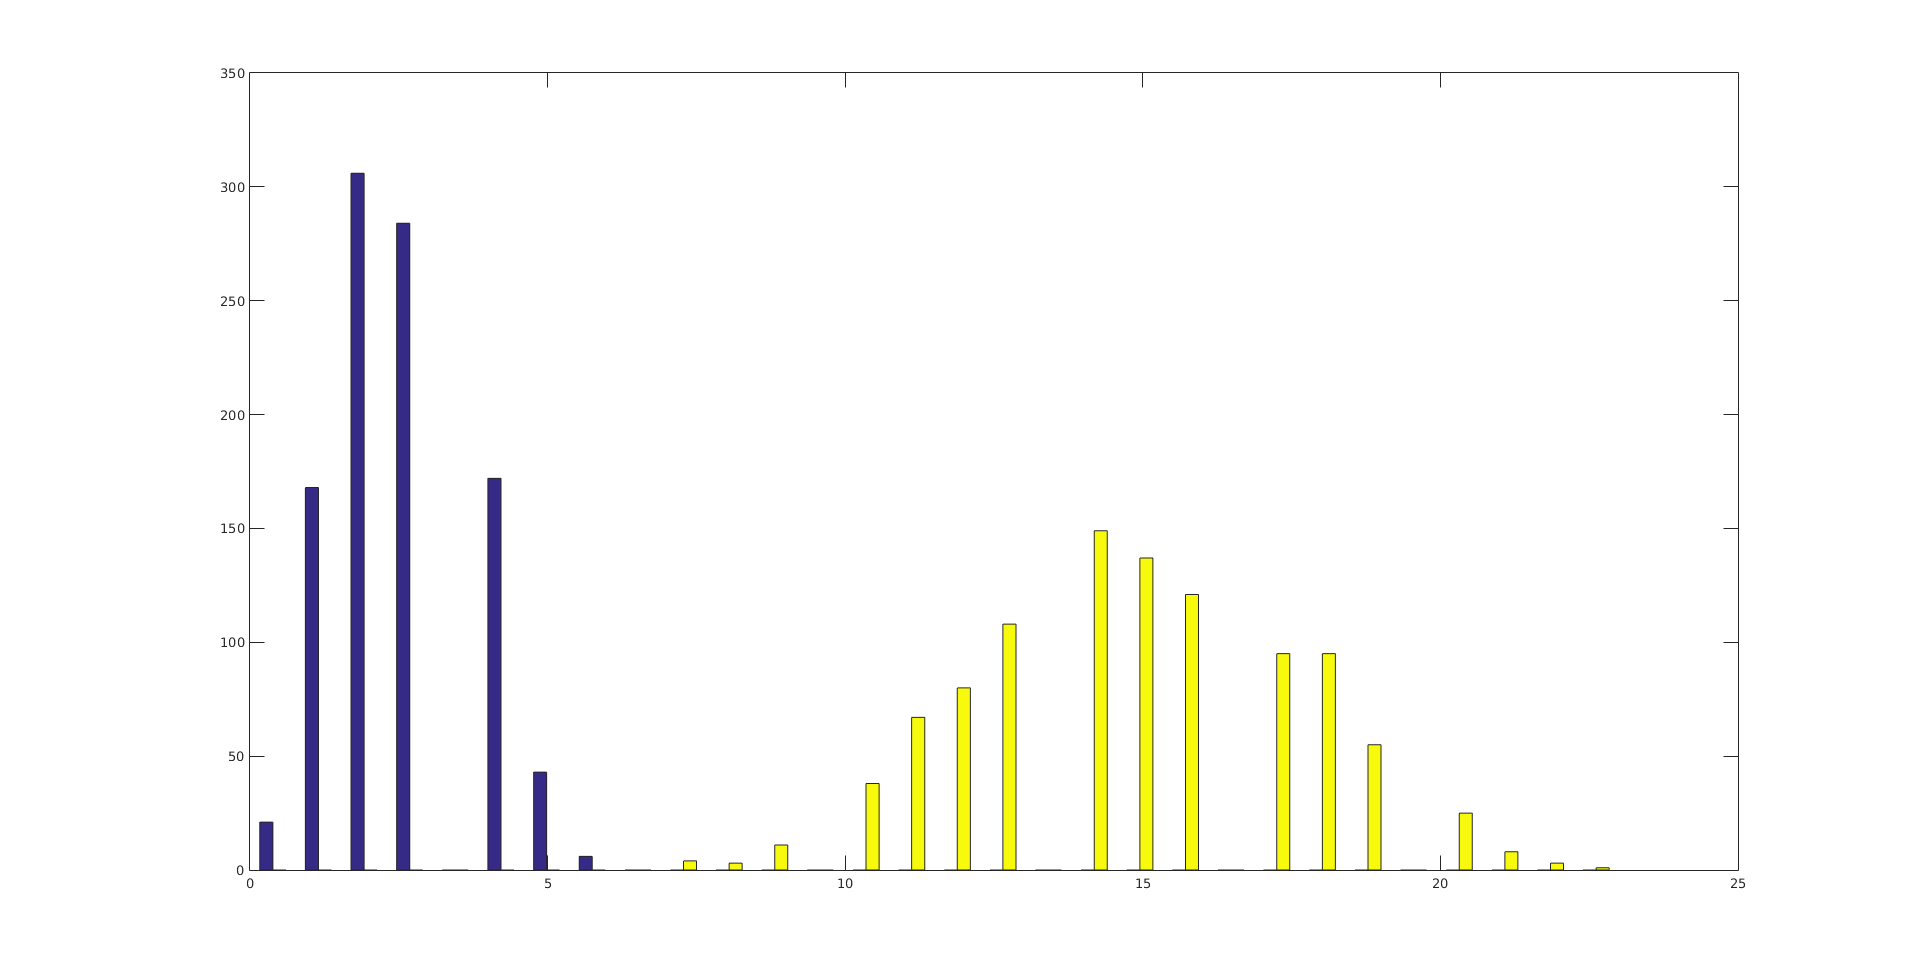
\includegraphics[width=\linewidth]{plot2_4.png}
\label{fig1.4b}
\end{figure}
\subsection{}
\subsection{}
\subsection{}
\subsection{}
\end{document}
